\documentclass[11pt]{article}
\usepackage[margin=1.15in]{geometry}
\usepackage{amsmath,amssymb}
\usepackage{graphicx}
\usepackage{booktabs}
\usepackage[hidelinks]{hyperref}
\usepackage{microtype}

\newcommand{\hid}{h_{\mathrm{id}}}
\newcommand{\Xmax}{X_{\max}}

\title{Independent computation of the 2D Boussinesq corner blowup profile:\\
the scaling exponent, an eigenvalue-free stability certificate,\\
and a free-residual test that catches a false root}

% TODO(author): confirm the form of the name and add affiliation before posting.
\author{J.~Hill}
\date{28 July 2026}

\begin{document}
\maketitle

\begin{abstract}
We compute the self-similar blowup profile of the 2D Boussinesq system in a corner
domain, the object underlying the Luo--Hou scenario for 3D axisymmetric Euler with
boundary, by a route independent in discretization, formulation and solver from both
existing computations. The profile is solved as a root problem with an explicit sparse
Jacobian, rather than by marching or by neural approximation. We obtain
$\alpha = -0.34240 \pm 4.4\times10^{-5}$, consistent with the cross-method reference
value $-0.34240009$, which is itself agreed on by an adaptive-mesh march and a
physics-informed network to $3.4\times10^{-7}$. The free gauge residual, a functional
the solve is answerable to nothing for, closes to $1.8\times10^{-6}$ on the quoted
ladder and to $8.7\times10^{-7}$ at the deepest corner resolution reached.

Our independence is not total, and we state the exception precisely: two scalar corner
constants, $W_x$ and $\Theta_{xx}$, are read off the reference profile and imposed as
gauge targets, and the interior seed of the production ladder is interpolated from the
same profile. We show the \emph{seed} dependence is immaterial (Section~\ref{sec:axes})
and that the \emph{corner constants} are not: freeing one of them moves $\alpha$ by
$9.7\times10^{-5}$, about twice the quoted bar. This is a genuine shared input, not an
independent check, and the note treats it as such throughout.

Three further results are, to our knowledge, new. First, the corner-regularized system
possesses an exact one-parameter scaling symmetry under which $\alpha$ is invariant; we
verify it symbolically and confirm on the converged root that the Jacobian annihilates
its generator on every covariant row to $2.8\times10^{-12}$. Second, we certify linear
stability of the profile \emph{without trusting any eigenvalue}, by a Lyapunov
certificate on the descriptor realization whose verification reduces to an absolute
inequality; in the same section we show the rightmost eigenvalue of this operator is
unconverged as a discretization at both resolutions computed, agreeing between two
solution routes to $7.2\times10^{-9}$ while disagreeing between two grids by
$2.1\times10^{-1}$. Third, we report a \emph{false} root: a state converging to
$\|F\| = 5.4\times10^{-14}$, distinct from the ground state, stable under wedge
truncation, and morphologically coherent, which is nevertheless an artifact of the
pinned discretization. We give the one-line diagnostic that separates it from the true
profile at three orders of magnitude, and argue that residual, distinctness, parameter
stability and morphological coherence are jointly insufficient to certify a
self-similar profile.
\end{abstract}

\section{The object and the prior art}

The Luo--Hou scenario~\cite{luohou} proposes finite-time blowup for 3D axisymmetric
Euler with a solid boundary, driven by a hyperbolic point on the wall. Its 2D
Boussinesq analogue admits a self-similar reduction whose profile satisfies a nonlinear
elliptic system in a corner. The quantity of interest is the scaling exponent $\alpha$,
which fixes the temporal rate of the blowup.

Two computations of this profile exist. Chen and
Hou~\cite{chenhou1,chenhou2,chenhou3} solve it by an adaptive-mesh march with a slaved
gauge, in the line of work supporting a computer-assisted proof. Wang and
collaborators~\cite{deepmind} solve it with a physics-informed network refined by
Gauss--Newton~\cite{thesis}. The two share neither discretization nor solution
strategy, and they agree on $\alpha$ to $3.4\times10^{-7}$, which is why we treat
$\alpha_{\mathrm{ref}} = -0.34240009$ as a reference rather than as a competitor.

What has been missing is a third route with a different failure mode. A march
accumulates error along its direction of integration; a network's error is opaque to
the practitioner. A root problem with an explicit Jacobian fails in neither of those
ways. It fails by rank deficiency, by inconsistency, or by converging to the wrong
object, all of which are detectable by linear algebra on matrices one can inspect.
Sections~\ref{sec:mechanisms} and~\ref{sec:false} are, respectively, an instance of the
second failure mode and an instance of the third, both caught by that inspection.

\section{Formulation}

\subsection{Corner regularization}

In the corner frame $\xi = \ln(1+r)$ with $\beta$ the angular variable on the wedge,
the natural unknowns carry algebraic prefactors at the corner. Working with them
directly produces transport rows that are $O(\xi)$-scaled near the wall, with the
consequences documented in Section~\ref{sec:dust}. We instead substitute globally
\[
  \tilde\Omega = \xi A, \qquad \tilde B = \xi^2 B, \qquad \tilde\Psi = \xi^2 P,
\]
and divide the three residuals by $\xi$, $\xi^2$, $\xi^2$, performing every
cancellation analytically rather than in floating point. Writing
$G_1 = -\mathrm{expm1}(-\xi)/\xi$ (analytic, $G_1(0) = 1$) and $E_1 = e^{a_0\xi}/G_1$,
and bundling the first-order operators as
\[
  L_A = I + X(D_\xi + a_0 I), \qquad
  L_{B2} = 2I + X\bigl(D_\xi + (1+2a_0)I\bigr), \qquad
  L_{P\mu} = 2I + X(D_\xi + \mu I),
\]
the divided residuals are exact identities. Three consequences follow, each closing a
failure mode of the undivided formulation. The corner circle $\xi = 0$ now carries real
equations rather than imposed identities. The wall-line rows are $O(1)$ instead of
$O(\xi)$. And the gauge constraints become single-entry value pins in place of
derivative functionals whose conditioning grew as $N^4$.

\subsection{Panels, and the decision that made the Jacobian sparse}

The radial direction is discretized by piecewise-Chebyshev panels with duplicated
interface nodes and classical patching: $C^0$ matching for the transport equations,
$C^0$ and $C^1$ for the Poisson equation.

The load-bearing choice is to keep $\tilde\Psi$ as an \emph{unknown} rather than
eliminating it by a Poisson solve. Elimination is the obvious move and it is a trap: it
makes every operator nonlocal, so the Jacobian is dense at any grid size, and each
Jacobian column costs a Poisson solve. Retaining $\tilde\Psi$ keeps every operator local
and the exact Jacobian sparse. Every diagnostic in this note is a sparse factorization,
so every result below depends on that choice.

\subsection{Gauge closure and the free residual}
\label{sec:free}

The scalars $c_\ell, c_w$ are closed by two gauge functionals evaluated at the corner,
with targets $W_x = 1.19620314$ and $\Theta_{xx} = 1.79819132$ read from the reference
profile. These two numbers are the note's one substantive shared input with prior work,
and Section~\ref{sec:cost} measures what they cost.

This closure leaves a functional \emph{unused}, and it is the most valuable object in
the computation. The continuum corner algebra forces
\[
  c_\ell = \frac{2\Theta_{xx}}{W_x} = 3.00649824,
\]
and nothing in the discrete system imposes it. We therefore define the \textbf{free
residual}
\[
  \hid \;=\; c_\ell - \frac{2\Theta_{xx}}{W_x},
\]
report it beside every converged solution, and treat it as the primary certificate. It
is answerable to no tuning. Section~\ref{sec:false} is the argument that a computation
of this kind should not be believed without such a functional.

\section{Two mechanisms found along the way}
\label{sec:mechanisms}

\subsection{Corner dust}
\label{sec:dust}

Transport rows collocated at wall nodes with $\xi \lesssim 0.025$ are near-vacuous: in
the undivided formulation their entries are $O(\xi)$-scaled and drown in roundoff. The
rows go dependent and the system becomes rank-deficient and inconsistent.

This single threshold is consistent with a family of failures previously recorded as
unrelated: the dense solver's ceiling at $N \approx 52$ to $56$, the failure at panel
length $L = 10$, and an outlier at $N = 52$, all of which satisfy ``the first radial
node falls below $\xi \approx 0.025$'' while the successful configurations do not. The
regularization above removes the mechanism rather than avoiding it.

\subsection{The wedge truncation carries a singular layer}
\label{sec:layer}

Computations on this domain truncate the wedge by $\varepsilon_b$, replacing the opening
$\pi/2$ with $\pi/2 - 2\varepsilon_b$. This is not a small perturbation of the boundary
condition. It shifts the corner exponent to
\[
  k \;=\; \frac{\pi}{\pi/2 - 2\varepsilon_b},
\]
so that $P = \tilde\Psi/\xi^2$ carries a weakly singular layer $\xi^{k-2}$ that no
polynomial radial basis represents. At $\varepsilon_b = 10^{-3}$, $k = 2.002550$.

The observable consequence is sharp and was initially baffling. Coarse corner panels
cannot resolve the misfit and converge normally. Once the first radial node drops below
roughly $0.012$, the layer is resolved and we can find no root: the residual floors at
$8\times10^{-5}$ to $1.4\times10^{-4}$ with every Newton step accepted and the residual
immobile, for two independent solvers. Reducing $\varepsilon_b$ to $10^{-4}$ removes the
floor entirely and the same configurations converge in three to four Newton steps.

This is worth stating plainly, because the symptom, a residual floor with accepted
steps, is easily misread as a solver defect. It is a statement about the truncated
problem.

\section{The exponent}

\subsection{The ladder and the quoted value}

At $\mathrm{degs} = (24,56,12)$, $N_\beta = 36$:

\begin{center}
\begin{tabular}{cccc}
\toprule
$\varepsilon_b$ & $\alpha$ & $\hid/c_\ell$ & $\|F\|$ \\
\midrule
$1.0\times10^{-4}$ & $-0.34541032$ & $+2.6\times10^{-5}$ & $9.4\times10^{-13}$ \\
$5.0\times10^{-5}$ & $-0.34386167$ & $+1.4\times10^{-5}$ & $6.4\times10^{-12}$ \\
$2.5\times10^{-5}$ & $-0.34312079$ & $+7.1\times10^{-6}$ & $5.3\times10^{-12}$ \\
$1.0\times10^{-5}$ & $-0.34268591$ & $+3.2\times10^{-6}$ & $3.9\times10^{-12}$ \\
$5.0\times10^{-6}$ & $-0.34254247$ & $+1.8\times10^{-6}$ & $7.3\times10^{-12}$ \\
\bottomrule
\end{tabular}
\end{center}

The free residual is reported relative to $c_\ell$; it falls monotonically to
$1.8\times10^{-6}$. At corner degree $28$ and $\varepsilon_b = 5\times10^{-6}$ it
reaches $8.7\times10^{-7}$, with $\alpha$ moving by $9.8\times10^{-6}$.

Extrapolating to $\varepsilon_b \to 0$ requires choosing a model class, and we decline
to choose. Three families fit the five-rung ladder with residuals we cannot distinguish
on five points (Figure~\ref{fig:ladder}):

\begin{center}
\begin{tabular}{lcc}
\toprule
model & $\alpha(0)$ & deviation from reference \\
\midrule
$a + b\varepsilon$ & $-0.34237665$ & $+2.3\times10^{-5}$ \\
$a + b\varepsilon + c\varepsilon^2$ & $-0.34240048$ & $-3.9\times10^{-7}$ \\
$a + b\varepsilon + c\,\varepsilon\ln\varepsilon$ & $-0.34241599$ & $-1.6\times10^{-5}$ \\
\bottomrule
\end{tabular}
\end{center}

Their spread is $3.93\times10^{-5}$ about a midrange of $-0.34239632$. Since the
singular layer of Section~\ref{sec:layer} has exponent $k - 2 \sim \varepsilon_b$, a
non-polynomial term is physically plausible and the polynomial fit cannot be preferred
on principle. Adding in quadrature the measured corner-degree systematic of
Section~\ref{sec:axes} ($1.94\times10^{-5}$) gives the quoted bar:
\[
  \boxed{\;\alpha = -0.34240 \pm 4.4\times10^{-5}\;}
\]

We note, without adopting it, that the extrapolation stabilizes as the coarsest rungs
are dropped: the linear and quadratic fits differ by $2.4\times10^{-5}$ on all five
rungs, $7.2\times10^{-6}$ on the deepest four, and $2.5\times10^{-6}$ on the deepest
three. Quoting the deepest-three bar would report agreement at $2.5\times10^{-6}$. We do
not, because choosing the subset that tightens the bar is the same error as choosing the
model family that does.

\begin{figure}[t]
\centering
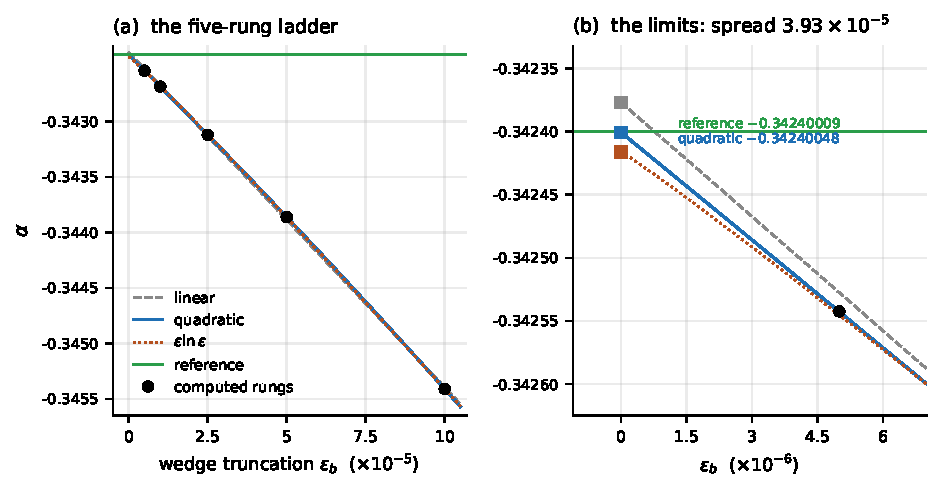
\includegraphics[width=\textwidth]{fig/fig1_ladder.pdf}
\caption{The five-rung $\varepsilon_b$ ladder (a) and, resolved in (b), the
$3.93\times10^{-5}$ spread between the three extrapolation families at
$\varepsilon_b \to 0$, against the cross-method reference value. Every plotted point is
a converged solve.}
\label{fig:ladder}
\end{figure}

\subsection{Which axes were probed, and how far}
\label{sec:axes}

\begin{center}
\begin{tabular}{lll}
\toprule
axis & worst effect on $\alpha$ & status \\
\midrule
$N_\beta$, $36 \to 48$ & $1.16\times10^{-8}$ & closed \\
seed provenance & $9.65\times10^{-8}$ & closed \\
axis-column pinning & $3.0\times10^{-8}$ & closed \\
far-field truncation, $\Xmax\ 25 \to 32$ & $1.45\times10^{-10}$ & closed \\
middle panel edge, $15 \to 18$ & $1.45\times10^{-10}$ & closed \\
corner degree, $24 \to 28$ & $1.94\times10^{-5}$ & in the bar \\
corner degree, $16 \to 24$ & $6.98\times10^{-4}$ & not converged at 16 \\
$\varepsilon_b$ truncation & extrapolated, layer analysed & in the bar \\
\bottomrule
\end{tabular}
\end{center}

Two entries need comment.

The seed row closes the last hidden constant. Every configuration in the production
ladder seeded its interior field by interpolating the reference profile, and agreement
among configurations is structurally blind to anything they all share. We re-solved from
three \emph{purely analytic} seeds carrying no reference data in the interior, namely the
corner limits times $e^{-\xi/L}$ for $L = 2, 4, 8$, obtaining deviations
$9.7\times10^{-8}$, $7.8\times10^{-8}$ and $6.9\times10^{-8}$ with a spread among
themselves of $2.7\times10^{-8}$. The $L = 1$ seed did not converge, terminating with
zero accepted Newton steps, which we report as a basin observation. These runs were
performed at a configuration where $\alpha$ itself is about $0.7\%$ from the extrapolated
value, so they bound the seed sensitivity of the \emph{root found}, not of the
extrapolated exponent.

The far-field and panel-edge rows were the final open axes. Moving the far field from
$\Xmax = 25$ to $32$, and independently moving the middle panel edge from $15$ to $18$,
changes $\alpha$ by $1.45\times10^{-10}$ in both cases, five orders below the quoted bar.
We verified the interventions were real rather than ignored: the radial node sets differ
by $7.0$ and $3.0$ respectively, so the insensitivity is a property of the solution and
not of the driver.

\subsection{What the shared corner constants cost}
\label{sec:cost}

Freeing $\Theta_{xx}$ as an unknown and closing the system with the corner identity (the
experiment of Section~\ref{sec:rescue}, which fails for an unrelated reason) moves the
converged $\alpha$ by $9.73\times10^{-5}$, about twice the quoted bar. The gauge targets
are therefore a real shared input with Chen and Hou, and this note claims independence of
\emph{method}, not of \emph{data}.

\section{The exact scaling symmetry}
\label{sec:symmetry}

The divided residuals are covariant under
\[
  A \to sA, \quad B \to s^2 B, \quad P \to sP, \quad c_\ell \to s\,c_\ell,
  \quad c_w \to s\,c_w,
\]
with $R_\Omega' \to s^2 R_\Omega'$, $R_B' \to s^3 R_B'$, $R_P' \to s R_P'$. The grading
$(1,2,1,1,1)$ is the unique solution; the system is \emph{not} homogeneous under field
scaling alone, and the compensating rescale of $(c_\ell, c_w)$ is what makes
$\alpha = c_w/c_\ell$ \textbf{invariant}.

Verification is at two levels. Symbolically the identities hold exactly. On the coded
solver at a random state, all $896$ covariant rows scale with their derived exponent to
$1.348\times10^{-15}$, and the Euler check $Jv = d\,F$ holds to $1.011\times10^{-15}$;
the only rows that break covariance are the static pins and gauge targets, and their
breakage equals $(s^k - 1)\times\text{field}$ to $4.441\times10^{-16}$, as predicted.

At a converged root the consequence is structural. Euler's identity gives
$DR\cdot v = d\,R$ for a row of degree $d$, and $R = 0$ at a root, so $Jv = 0$ on every
covariant row. Measured on the converged profile with generator
$v = (A, 2B, P, c_\ell, c_w)$:
\[
  \|Jv\|_{\text{covariant}} = 2.814\times10^{-12},
  \qquad
  \frac{\|Jv\|_{\text{pins+gauge}}}{\|Jv\|} = 100.0000\%.
\]
The symmetry is therefore the dominant soft direction of the Jacobian at the solution:
$\sigma_{\min}(J) = 2.536\times10^{-6}$, with the soft mode $68.9\%$ aligned with $v$.
The gauge rows suppress its $c_\ell, c_w$ components to $0.305$ and $0.646$ of the
predicted values, which is why the mode presents in parameter sweeps as
``$c_\ell, c_w$ nearly fixed'' and was for some time misread as such.

\section{Linear stability, without trusting an eigenvalue}

\subsection{The realization}

The stability operator is not the Jacobian of the steady system. In the divided variables
the exponential factors are independent of the self-similar time, so the mass matrix on
the two transported blocks is the identity and the linearization is a \textbf{descriptor
pencil} $(E, J)$ with $J$ the solver's own Jacobian unmodified and $E$ a $0/1$ diagonal
mask, equal to $1$ exactly on live transport rows. Everything else, the pins, the
interface matching, the Poisson block, the two gauge rows and the two scalar columns, is
algebraic. The pencil has Hessenberg index $2$. On a reduced structural configuration
($N = 722$) a QZ count returns $376$ finite and $346$ infinite eigenvalues, the infinite
count matching $(N - \operatorname{rank}E) + m$ exactly, and the compressed generator
agrees with the pencil to $3.7\times10^{-10}$.

The admissible state space is $\ker C_g$. Restricting to it removes the grading direction
\emph{by construction}:
\[
  \sigma_{\min}(J) = 2.5356\times10^{-6}
  \;\longrightarrow\;
  \sigma_{\min}\!\left(L\big|_{\ker C_g}\right) = 3.9701\times10^{-3},
\]
a factor of $1565.7$, reproduced at three roots ($1565.7$, $1724.0$, $1529.1$; these
roots have $\alpha = -0.34471$, $-0.34541$, $-0.34349$, none of them the quoted
extrapolated value) with gauge leakage $\|C_g w\|/\|w\| = 3.9\times10^{-17}$.

We record a negative result about our own first instinct. Deflating the grading direction
explicitly, which we expected to be necessary, is \emph{wrong} rather than redundant. Its
restricted shadow is an ordinary stiff direction of the generator,
$\|Lw_1\|/\|w_1\| = 12.08$, about $1\%$ of $\|L\|$ and $3043\times$ $\sigma_{\min}(L)$,
and deflating it moves the resolvent norm in the right half plane by $19.6\%$.

\subsection{The certificate}

Since Section~\ref{sec:notmeas} shows this operator's eigenvalues are unconverged, we
certify stability without them. Solving $L^{\mathsf T}P + PL = -I$ by Bartels--Stewart
gives relative residuals $4.85\times10^{-16}$, $4.88\times10^{-16}$,
$4.68\times10^{-16}$ at three roots, with $\operatorname{chol}(P)$ succeeding at all
three.

We are explicit that Bartels--Stewart computes a real Schur decomposition internally, so
the route is not eigenvalue-free as an \emph{algorithm}. It is eigenvalue-free as a
\emph{certificate}, and the distinction is the point: verification does not require
trusting the Schur output, because the residual bound
\[
  \|E\|_2 \le 4.85\times10^{-16}\,\lambda_{\max}(P)\,\|L\| = 3.06\times10^{-8} < 1
\]
makes $P \succ 0$ with $L^{\mathsf T}P + PL \prec 0$ an inequality checkable
independently. Hurwitz-ness follows from that inequality, not from any computed
eigenvalue.

The companion pseudospectral statement is that no $\varepsilon$-pseudospectrum reaches
$\operatorname{Re}z > 0$ below $\varepsilon^* = 3.93\times10^{-3}$ at the first
resolution and $3.08\times10^{-3}$ at the second, against a round-off floor
$n\varepsilon_{\mathrm{mach}}\|L\| = 1.175\times10^{-9}$. We quote the \emph{worst}
margin, $8.8\times10^{5}$. The right-half-plane minimum sits on the imaginary axis
($3.946\times10^{-3}$ against $8.984\times10^{-3}$ over the interior), as
Davies--Shargorodsky requires. The verdict survives the refinements available: $N_\beta$
from $36$ to $28$ moves the spectral abscissa by $1.56\times10^{-6}$ and $\Xmax$ from
$25$ to $18$ by $3.36\times10^{-5}$. The $\varepsilon^*$ level does not survive, moving
$21.5\%$ across corner degrees, and is quoted with that band.

One caveat is structural rather than numerical: the untruncated essential spectrum of
this operator sits on the imaginary axis, so $\varepsilon^*$ should be expected to shrink
as $\Xmax$ grows. Our $\Xmax$ pair above is a coarsening rather than a refinement, and
the behaviour of $\varepsilon^*$ under genuine far-field refinement is untested.

Transient growth is genuine: $89.7 \le \sup_t \|e^{tL}\| \le 5807.6$ at the first
resolution and $148.7$ to $7973.8$ at the second, in the raw collocation norm, which is
not similarity-invariant and is labelled as such.

Two quantities that look like physics are not. A single-dominant-block model of $L$
predicts $\omega(L)/\|L\| = 1/2$ exactly, and we measure $0.4952$, $0.4967$, $0.4952$;
the closed form $e^{a_0\xi}\xi/2$ matches to $5.140972\times10^{-1}$ against
$5.140981\times10^{-1}$, and zeroing that block caps the maximum real part at $+15.68$.
And the essential numerical range of the corner-regularized symbol is $\mathbb{C}$, not
the imaginary axis: $\max\operatorname{Re}W(S) = +5.14\times10^{4}$ at $k = 10^5$ and
$+5.14\times10^{5}$ at $k = 10^6$, growing linearly. Spectral pollution confinement is
vacuous in this norm. This retracts a closed-form essential-numerical-range claim made
earlier in this project.

\subsection{What is not converged, and what is not claimed}
\label{sec:notmeas}

The rightmost eigenvalue is agreed on by two independent computational routes to
$7.2\times10^{-9}$ (worst of two roots), and disagrees between two grids by
$2.1\times10^{-1}$, changing character from a complex pair to a real value. Seven and a
half orders of magnitude separate ``well-posed as linear algebra'' from ``converged as
discretization.'' The eigenvalue condition numbers are $1.1\times10^{3}$,
$2.3\times10^{3}$, $1.5\times10^{3}$. We report no eigenvalue, and we state the negative
in the form the evidence supports: unconverged as a discretization at the two resolutions
computed, not unmeasurable in principle.

We do not claim unconditional linear stability. The Lyapunov rate $8.82\times10^{-6}$
lies $3.6\times10^{4}$ below the Schur abscissa $3.17\times10^{-1}$: Hurwitz means no
right-half spectrum, not decay at a rate. The admissible class is corner-clamped, since
the corner pin removes the continuum two-dimensional corner ODE from the realization and
the axis column imposes an extra Dirichlet condition on the perturbation whose spectral
cost we have not measured. The claim is Hurwitz-ness of the corner-clamped linearization
at two resolutions, in the raw collocation norm, at fixed $\varepsilon_b$ on a truncated
wedge, and nothing larger.

\section{A false root}
\label{sec:false}

The following is reported because we believe it is the most transferable content in this
note.

\subsection{What it passed}

Searching for unstable branches, we froze the exponent at a published unstable value and
searched \emph{field} space by deflation. One start in eight, at half the ground state's
amplitude, converged to a state with $\|F\| = 5.4\times10^{-14}$ at relative distance
$1.70$ from the ground state. It passed three independent checks. It satisfied the corner
algebra to $0.1\%$. Its self-consistent exponent was stable under wedge truncation,
moving $1.3\times10^{-5}$ across the decade $\varepsilon_b = 10^{-4}$ to $10^{-5}$, where
the ground state moves $2.72\times10^{-3}$ over the same decade. And it carried a
coherent morphological signature, an outward-displaced amplitude lobe and a sign-flipped
angular harmonic at $6172\times$ the variation of the ground branch. By every test we had
been applying, it was a new solution.

\begin{figure}[t]
\centering
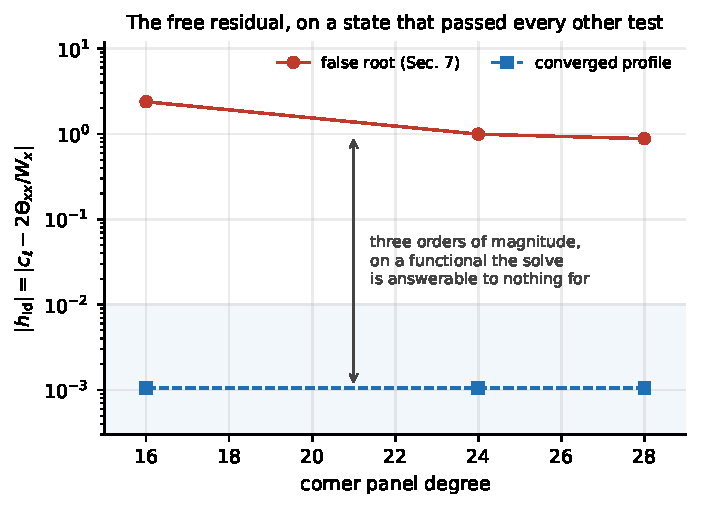
\includegraphics[width=0.72\textwidth]{fig/fig2_free_residual.pdf}
\caption{The free residual $|\hid|$ for the converged profile and for the false root,
across corner degree. Three orders of magnitude, on a functional neither solve is
answerable to, separating two states that agree on every other diagnostic.}
\label{fig:free}
\end{figure}

\subsection{What it was}

Under refinement its exponent moved \emph{away} from $\alpha_1$ with \emph{growing}
steps, and toward $\alpha_2$ and $\alpha_3$ without contracting on either
(Figure~\ref{fig:drift}):

\begin{center}
\begin{tabular}{lccc}
\toprule
resolution & $\alpha$ & $c_\ell$ & $\hid$ \\
\midrule
$(16,40,12)$ & $-0.42172919$ & $5.392$ & $+2.386$ \\
$(24,56,12)$ & $-0.42554621$ & $4.001$ & $+0.994$ \\
$(28,64,18)$ & $-0.43083651$ & $3.887$ & $+0.880$ \\
ground, for scale & $-0.34471229$ & $3.005$ & $-0.00106$ \\
\bottomrule
\end{tabular}
\end{center}

The free residual of Section~\ref{sec:free} is violated by $O(1)$ throughout, three
orders of magnitude above the ground state (Figure~\ref{fig:free}), while every other
diagnostic looks healthy. Its distance to $\alpha_2$ shrinks from $2.23\times10^{-2}$ to
$1.31\times10^{-2}$ across the three rungs, which is why we describe the object as
drifting rather than diverging, and why an ``$\alpha_2$ in disguise'' reading cannot be
excluded by these data alone.

\begin{figure}[t]
\centering
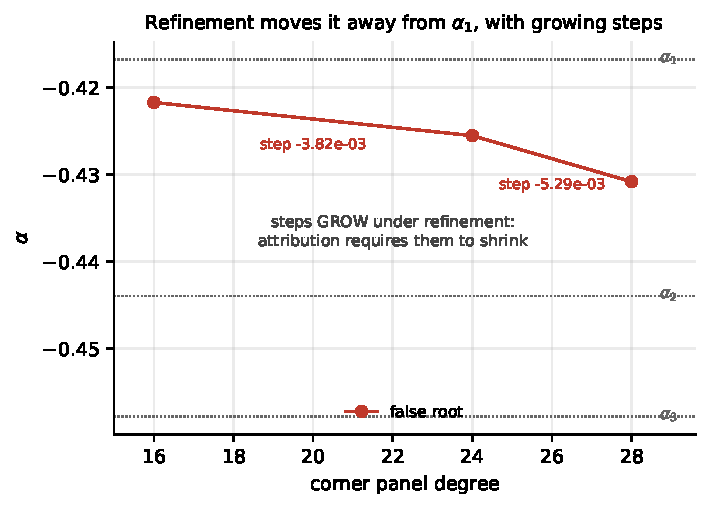
\includegraphics[width=0.72\textwidth]{fig/fig3_drift.pdf}
\caption{The false root's exponent under refinement, with the published
$\alpha_1, \alpha_2, \alpha_3$ marked and the step sizes labelled. Attribution to
$\alpha_1$ requires the steps to shrink; they grow.}
\label{fig:drift}
\end{figure}

\subsection{The rescue that failed, and what its failure measured}
\label{sec:rescue}

We tested the natural rescue, that the state is a genuine profile carrying its \emph{own}
corner data, by promoting $\Theta_{xx}$ to an unknown ($W_x$ absorbs the scaling
normalization of Section~\ref{sec:symmetry}) and closing with the corner identity. The
formulation was built and its Jacobian verified to $4.2\times10^{-11}$, and it failed its
ground-state control, which is the informative outcome: the pinned solution family
\emph{self-parallels} the identity line, $dc_\ell/d\Theta_{xx} = +1.677$ against the
identity slope $2/W_x = +1.672$, a $99.7\%$ cancellation. The corner identity cannot
serve as a closure; it is a diagnostic and only a diagnostic. The candidate state then
failed from both corner-data seeds, with residuals floored at $2.2$ to
$2.4\times10^{-3}$, and a continuation ramp showed the identity defect has no sign
crossing anywhere physical, extrapolating to three times the true corner value.

\subsection{The lesson}

We conclude the state is an artifact of the pinned discretization with no continuum
limit, and we state the general form of the lesson: \textbf{residual, distinctness under
deflation, parameter stability and morphological coherence are jointly insufficient to
certify a self-similar profile.} In this instance a free residual separated the cases
where those four did not, on a single artifact, at a cost of one extra line of output. A
formulation that pins its gauge to imported corner data can manufacture such a state; we
have not seen the failure mode reported.

\section{Reproduction and retractions}

\texttt{polar\_cornerreg.py} implements Section~2 and returns $\hid$ on convergence.
\texttt{polar\_spectrum.py} implements the Section~6.1 realization and its three gates;
the Section~6.2 and 6.3 certificates were computed by separate measurement scripts. The
three figures are generated from logged measurements by \texttt{repro/scripts/figures.py}
with no smoothing and no interpolated points. \texttt{ALPHA\_RESULT.md} is the full
campaign record and \texttt{NOTE\_CLAIMS.md} grades every claim in this note against its
evidence.

Every retraction made during this work is recorded rather than removed: a spectral mode
claim built on unconverged eigenvalues; a log-periodic extrapolation refused by model
selection; the essential-numerical-range claim retracted above; and a corner-angle
derivative $d\alpha/d\theta = +1.40$ per radian, which was the most expensive of the four
and was withdrawn when the slope proved formulation-dependent ($-2.8$ in the panel frame
against approximately $-30$ regularized). We regard the retraction record as part of the
result.

\section*{Open questions}

Four questions stand open. The corner-clamped admissible class of
Section~\ref{sec:notmeas} removes two directions whose dynamical content is unmeasured.
The mass matrix $E = I$ on transport rows rests on two independent derivations and a
reduction check but not on a third structurally different test; a short time-march
compared against $e^{tL}$ on the same perturbation would supply one. The behaviour of
$\varepsilon^*$ under genuine far-field refinement of the stability operator is untested.
And the unstable branches remain unconfirmed by any non-network method, including this
one: the route attempted here produced the artifact of Section~\ref{sec:false}, and a
formulation treating $\alpha$ as a Newton unknown with its own normalization on the
untruncated problem is the natural next attempt.

\begin{thebibliography}{9}

\bibitem{chenhou1}
J.~Chen and T.~Y.~Hou,
\emph{Stable nearly self-similar blowup of the 2D Boussinesq and 3D Euler equations with
smooth data I: Analysis},
arXiv:2210.07191.

\bibitem{chenhou2}
J.~Chen and T.~Y.~Hou,
\emph{Stable nearly self-similar blowup of the 2D Boussinesq and 3D Euler equations with
smooth data II: Rigorous Numerics},
arXiv:2305.05660; Multiscale Model.\ Simul.\ \textbf{23}(1), 25--130 (2025).

\bibitem{chenhou3}
J.~Chen and T.~Y.~Hou,
\emph{Singularity formation in 3D Euler equations with smooth initial data and boundary},
Proc.\ Natl.\ Acad.\ Sci.\ USA (2025), doi:10.1073/pnas.2500940122.

\bibitem{deepmind}
Y.~Wang et al.,
\emph{Discovery of Unstable Singularities},
arXiv:2509.14185.

\bibitem{thesis}
Y.~Wang,
\emph{Singularity Formation: Synergy in Theoretical, Numerical and Machine Learning
Approaches},
arXiv:2604.16842 (PhD thesis).

\bibitem{luohou}
G.~Luo and T.~Y.~Hou,
\emph{Potentially singular solutions of the 3D axisymmetric Euler equations},
Proc.\ Natl.\ Acad.\ Sci.\ USA \textbf{111}(36), 12968--12973 (2014),
doi:10.1073/pnas.1405238111.

\end{thebibliography}

\end{document}
